
\chapter{Data}
\label{sec:Data Distribution}


Since the heat load image data was taken from real experiments, the data set is not uniform in the distribution of $\bar{\iota}$ values, which is shown in figure \ref{fig:data:iota_dist}. This means the distribution the network is attempting to learn is not uniform, or more explicitly, it's multimodal. This is a common problem in machine learning and is often addressed by using a loss function that is robust to multimodal distributions. The loss function used in this case is the $rmse$ \ref{eq:rmse}. The $rmse$ is a common loss function for regression problems, but it is not entirely robust to multimodal distributions. This was address by M. Blatzheim et al. \cite{Blatzheim_2018} by using simulated input data that provided a continuos extension to the output distribution.

\begin{figure}[htb]
	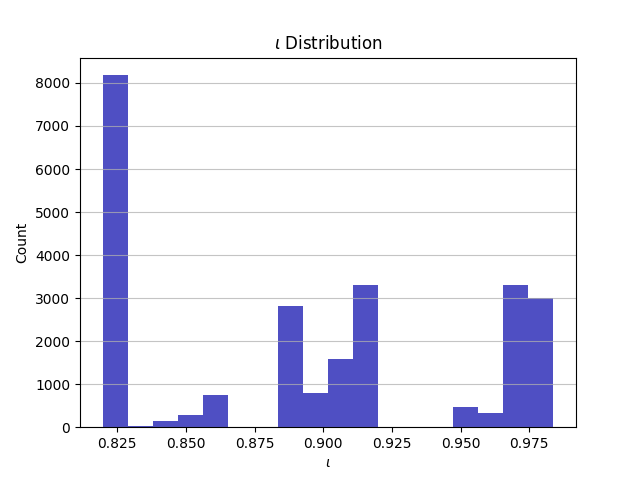
\includegraphics[width=\textwidth]{images/iota-dist.png}
	\caption{Distribution of simulated $\bar{\iota}$ values in the data set.}
	\label{fig:data:iota_dist}
\end{figure}

In an attempt to resolve the imbalanced distributions of the training, validation, and test sets were chosen to be as uniform as possible. This was challenging because the data is broken up into 42 different runs, or program numbers. Each program numbers will have highly correlated data so mixing data from program numbers that are included in the test and validation set could serve to pollute the metrics used to evaluate overfitting or hyperparameter tuning. Overfitting occurs when the model learns patterns in the training data that do not generalize to new data, leading to poor performance on the validation or test set. Since the training set requires the most data, the remaining test and validation sets cannot include more than a few runs.

\label{sec:Data Selection}

Since a program numbers covers several minutes of data collection, the images can exhibit a wide range of heat load patters and many samples my be unsuitable for training. For example, fig. \ref{fig:data:heat_load1} is an example of two heat load images from different timestamps, one early in the experiment and one later in the experiment with higher integrated heat load. The experimental conditions are low $\bar{\iota}$, high heating power, and a low density plasma. Fig. \ref{fig:data:heat_load2} is again two heat load images from different timestamps, this time both from program number 20180927.18, which had high $\bar{\iota}$, low heating power and high density. While the later timestamps for both set of images look dramatically different, with visible heat load patterns and different intensities, the early timestamp images for both pairs are visually indistinguishable. The plasma in the in both early examples had yet to deposit enough heat on the divertor to be resolved by the thermal cameras.

\begin{figure}[htb]
	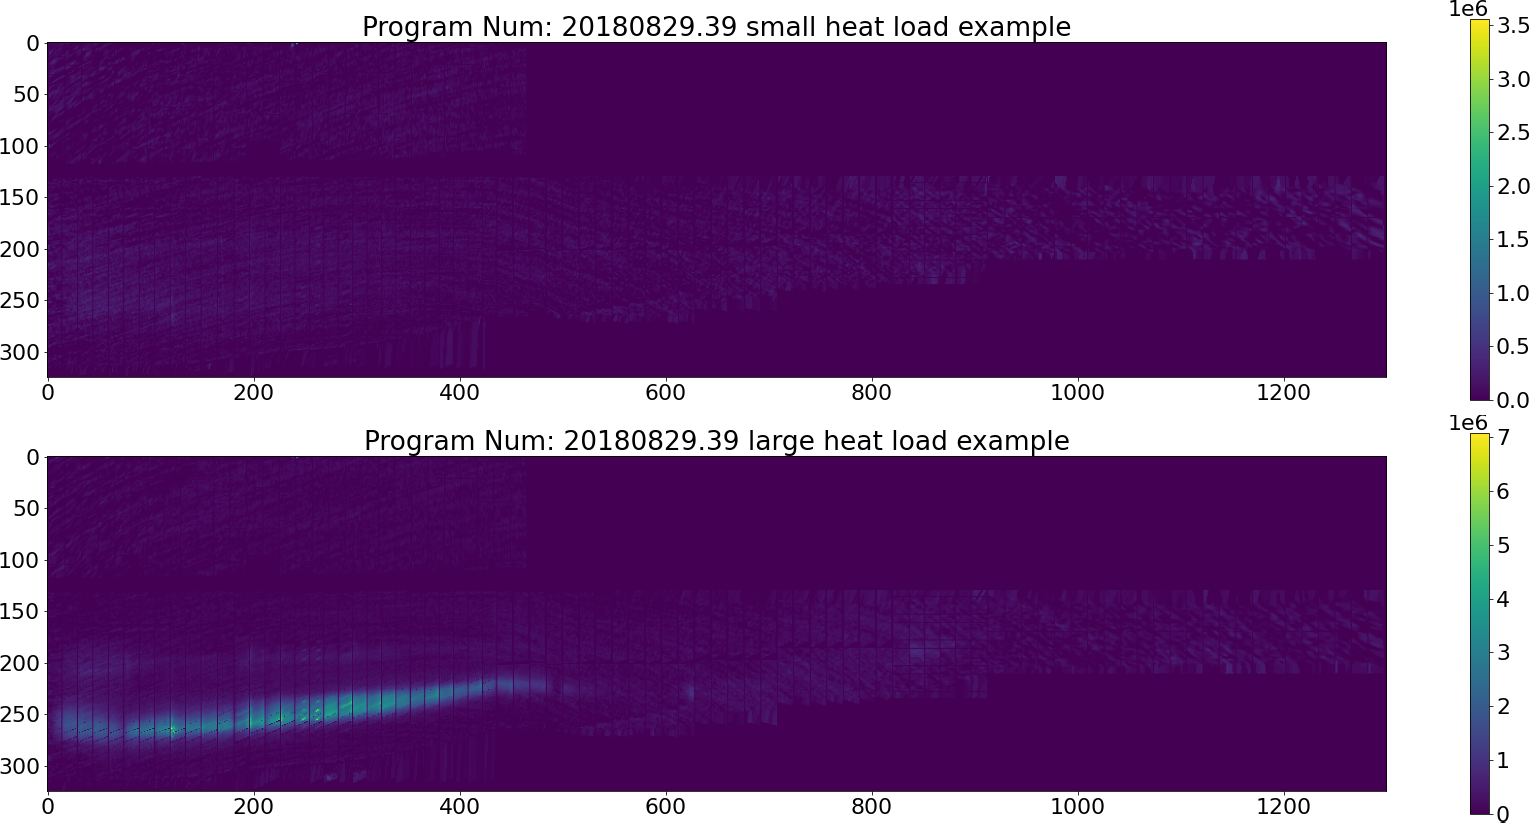
\includegraphics[width=\textwidth]{images/heat_load1.png}
	\caption{An example heat load image. Experimental conditions: low $\bar{\iota}$, high heating power, low density}
	\label{fig:data:heat_load1}
\end{figure}

\begin{figure}[htb]
	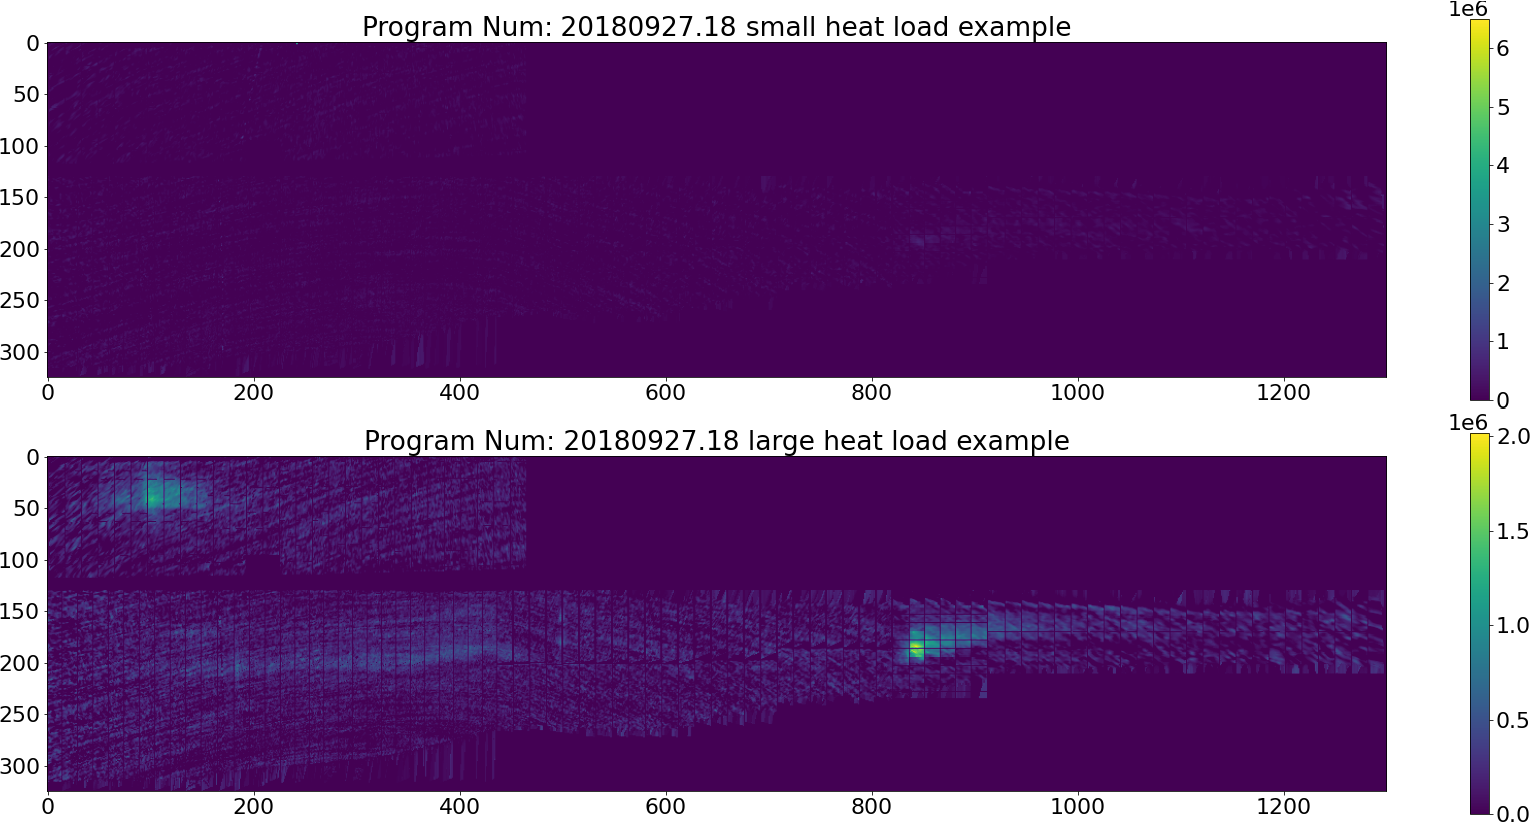
\includegraphics[width=\textwidth]{images/heat_load2.png}
	\caption{An example heat load image. Experimental conditions: high $\bar{\iota}$, low heating power, high density}
	\label{fig:data:heat_load2}
\end{figure}

To filter the unsuitable images, a variety edge cases were hand picked, both unsuitable and suitable examples. The edge cases were then used to create a filter that was applied to the data set. The filter applied a 24x24 2-dimensional convolutional kernel of ones (a 24x24 matrix of ones) to the image, effectively summing the values in a 24x24 pixel window to reduce the contributions from noise. A mask was created and only pixel values above the threshold were kept and the heat load from the unmasked pixes was integrated. A second threshold was selected and only images with an integrated heat load above the threshold were kept. The resulting images were then used to train the network. The two threshold values were selected to keep as much suitable data as possible while excluding as much unsuitable data as possible. The thresholds were hand tuned but could be automated by using a grid search to find the optimal values in the future. Since the amount of data included or excluded by this process was not significant, the hand tuned values were used as they were easier to implement.